%%%%%%%%%%%%%%%%%%%%%%%%%%%%%%%%%%%%%%%%%%%%%%%%%%%%%%%%%%%%%%%%%%%%%%%%%%%%%%%%%%%%%%%%%%%%%%%%%%%
%%%%%%%%%%%%%%%%%%%%%%%%%%%%%%%%%%%%%%%%%%%%%%%%%%%%%%%%%%%%%%%%%%%%%%%%%%%%%%%%%%%%%%%%%%%%%%%%%%%
\chapter{''Resultados''}

Visually, Rapid Eye Movement (REM) sleep is characterized by REMs, muscle atonia and 
desynchronized EEG activity. When quantitative analyses of the signals are carried out, usually, 
non-linearity and non-stationarity are assumed without an adequate analysis, especially in 
Old Adults (OA). Among the “weak” stationarity tests, the Priestley-Subba Rao (PSR) test 
calculates a “local” spectra that is “valid” only for punctual moments in time. A series of 
“smoothed” frequency filters give information of the time the local spectra is calculated. 
In here, weak REM sleep stationarity by the PSR test was compared to that from Wakefulness (W) 
and Non-REM (NREM) sleep. Methods:  8 Old Adults (OA) 
(age: 67.6 $\pm$ 5.7; education: 8.8 $\pm$ 2.6) 
without depression neither anxiety and with intact daily living activities were selected. Also, 
evaluations with the Mini-Mental State Examination (MMSE, 28.1 $\pm$ 1.8) and a one night 
polysomnography were performed. 30 second epochs were classified according to the AASM and every 
epoch of W, NREM and REM sleep was subjected to PSR tests. Percentages of stationary epochs were 
obtained with respect to the total number of epochs of each stage and Student t-tests were used 
to compare them. Results: The PSR effectively showed different proportions of stationarity 
according to the classification of stages in each subject. In Figure 1, in one OA, epochs with 
stationarity are shown in black and the classification of REM sleep is shown in green. Clearly, 
a lower proportion of stationarity was found in REM sleep vs the other stages. These differences 
reached significance in F7, Fp2, LOG and ROG (p $<$ 0.05, Figure 2). Conclusions: In OA, REM sleep 
showed lower proportions of epochs with stationarity vs. W and NREM sleep at anterior areas, a 
result that could be explained by the tonic and phasic REM sleep. When stationarity measurements 
are planned, it is recommended to differentiate anterior from lateral and posterior areas.

%%%%%%%%%%%%%%%%%%%%%%%%%%%%%%%%%%%%%%%%%%%%%%%%%%%%%%%%%%%%%%%%%%%%%%%%%%%%%%%%%%%%%%%%%%%%%%%%%%%

\section{Resultados del test PSR}

(Por ahora est\'a copiado y pegado un reporte preeliminar sobre los resultados
para tenerlo en cuenta y no olvidarlo; m\'as adelante
escribir\'e una explicaci\'opn adecuada.

Desde el punto de vista formal, se sigue directamente de la descripci\'on del test PSR, y s\'olo
hace falta indicar c\'omo se acomodaron los datos. Desde el punto de vista fisiol\'ogico es m\'as
interesante y extensa la parte que falta.)

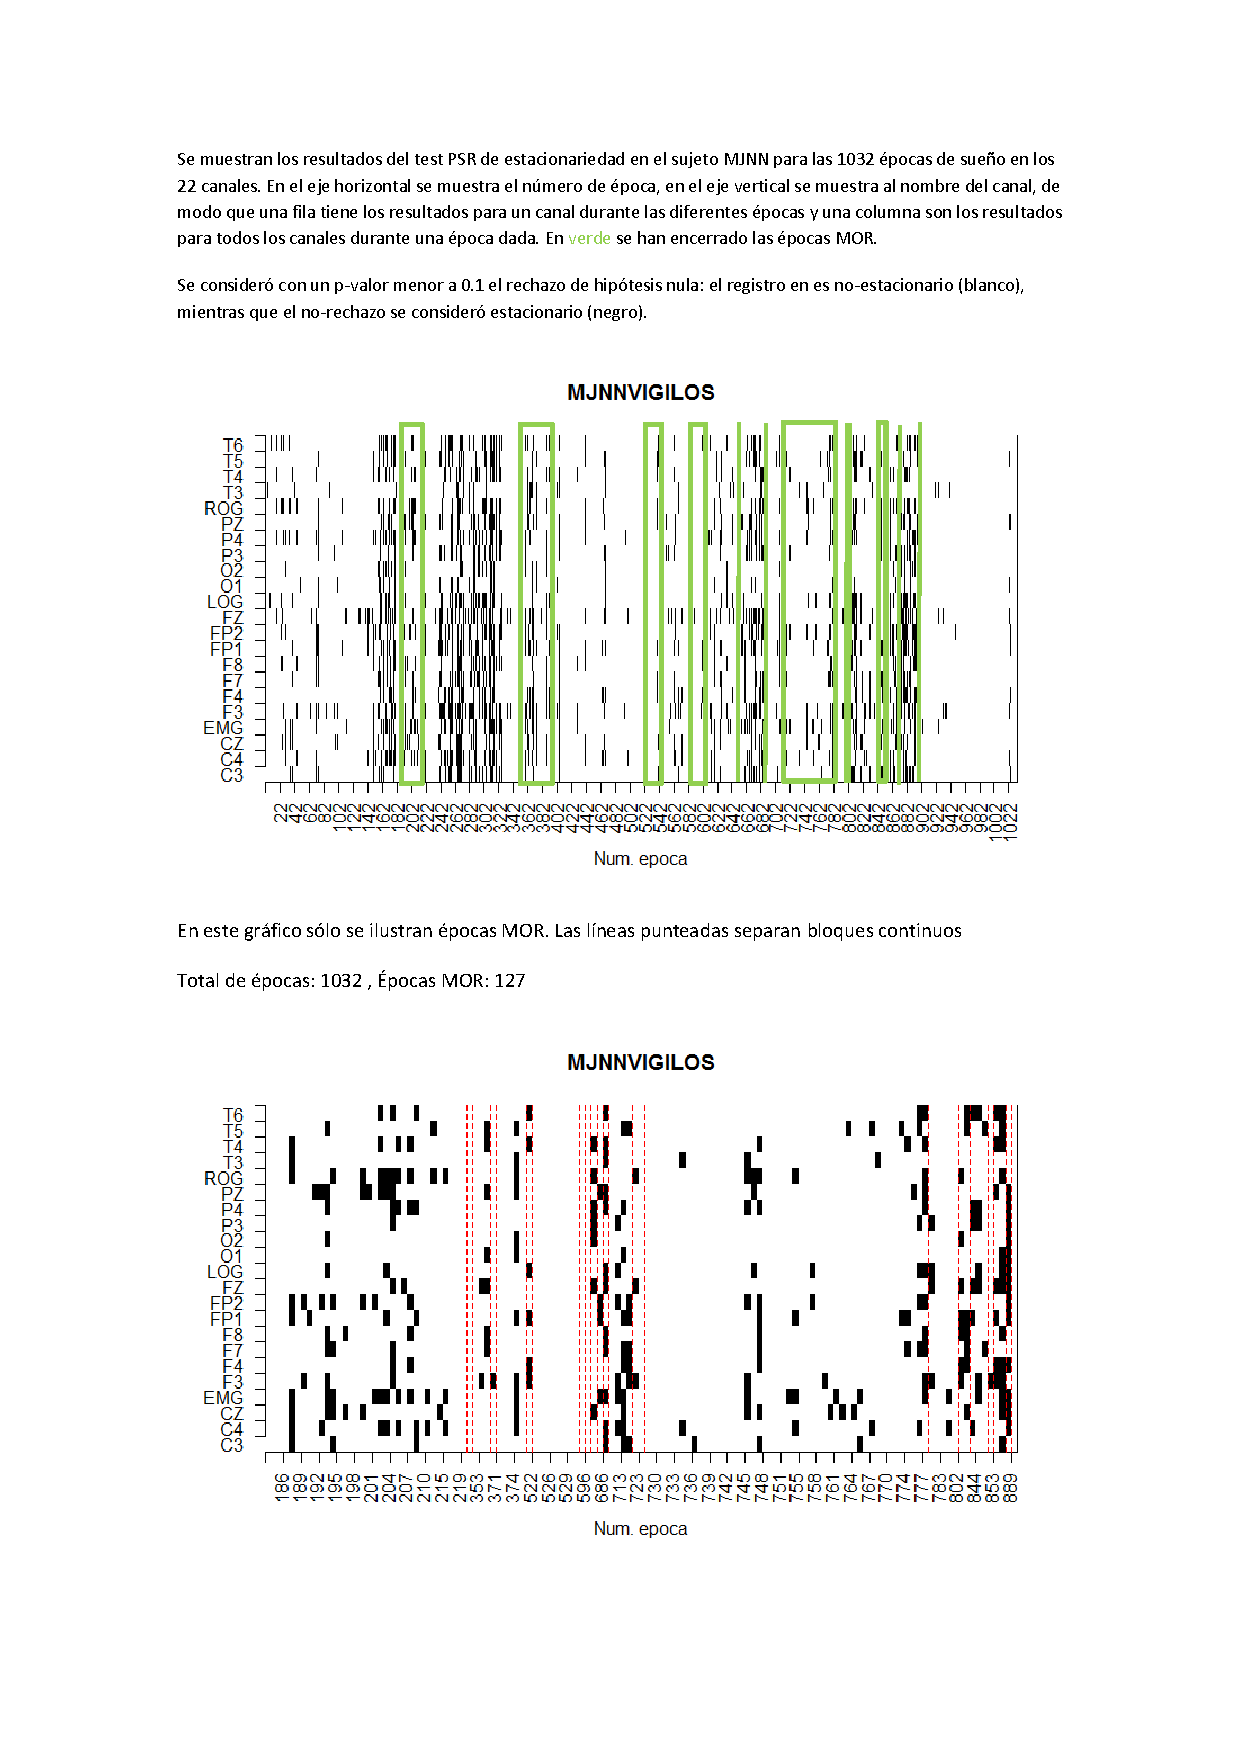
\includepdf[pages={1-},scale=.85]{reporte_de_estacionariedad_170120.pdf}

%%%%%%%%%%%%%%%%%%%%%%%%%%%%%%%%%%%%%%%%%%%%%%%%%%%%%%%%%%%%%%%%%%%%%%%%%%%%%%%%%%%%%%%%%%%%%%%%%%%
%%%%%%%%%%%%%%%%%%%%%%%%%%%%%%%%%%%%%%%%%%%%%%%%%%%%%%%%%%%%%%%%%%%%%%%%%%%%%%%%%%%%%%%%%%%%%%%%%%%